\documentclass[a4paper, 12pt, titlepage]{article}

% osnovni paketi za jezik in kodiranje znakov
\usepackage[slovene]{babel} 
\usepackage[utf8]{inputenc}
\usepackage[T1]{fontenc}
\usepackage{lmodern}

% dodatni paketi
\usepackage{amsmath, amssymb, amsthm}
\usepackage[font=small, center]{caption}
\usepackage[hidelinks]{hyperref}
\usepackage{graphicx}
\usepackage{wrapfig}
\usepackage{float}     
\usepackage{geometry}
\geometry{tmargin=1.5in, textwidth=6.5in}
\usepackage[table]{xcolor} % http://ctan.org/pkg/xcolor
\usepackage{biblatex}
\addbibresource{literatura.bib}

% priprava strani
\pagestyle{headings}

\begin{document}

\begin{titlepage}
    \begin{center}
        \large
        Fakulteta za matematiko in fiziko\\
        \vspace{8cm}
        \Huge
        \textbf{Računanje določenega integrala s trikotniki} \\
        \vspace{7cm}
        \large
        Terezija Krečič\\
        Pedagoška matematika\\
        \vspace{1cm}
        Mentor: Uroš Kuzman\\
        \vspace{0.5cm}
        Ljubljana\\
        ?. ?. 2023
    \end{center}
\end{titlepage}

\tableofcontents
\newpage

%%%%%%%%%%%%%%%%%%%%%%%%%%%%%%%%%%%%%%%%%%%%%%
\section{Uvod}

Naj bo $ f: [a,b] \rightarrow \mathbb{R} $ zvezna in pozitivna funkcija. Ploščino pod njenim grafom tipično aproksimiramo z Riemannovo vsoto oz. pravokotniki, da v limiti dobimo vrednost $ \int_{a}^{b}f(x)dx $. V nalogi si bomo ogledali metodo, ki integral konveksnih funkcij izračuna s pomočjo trikotnih območij.

????? Naš pristop temelji na generiranju goste \footnote{definicija: Množica D je \emph{gosta} v topološkem prostoru X natanko tedaj, kadar je presek množice D z vsako neprazno odprto podmnožico v X neprazen. V našem primeru to pomeni, da se v vsakem odprtem podintervalu intervala integriranja nahaja vsaj en element iz te podmmnožice.} podmnožice intervala, po katerem integriramo, preko neskončnega binarnega drevesa. To drevo generira vrsto, ki jo definira funkcija, ki jo integriramo, ter izbira vozlišč, zato lahko dobimo znano ali manj znano vrsto, za katero lahko vidimo, ali divergira ali konvergira in če, h kateri vrednosti. Še posebej zanimiv primer izhaja iz Stern-Brocot drevesa, ki izhaja iz enega tipa zeta funkcij.


\newpage
%%%%%%%%%%%%%%%%%%%%%%%%%%%%%%%%%%%%%%%%%%%%%%
\section{Motivacijski primer}

Za boljšo predstavo o ideji integracije preko trikotnikov si poglejmo konkreten primer funkcije $ f(x) = \frac{1}{x} $ na intervalu $ (0, \infty) $. Gosto podmnožico definicijskega območja $ (0, \infty) $ generirajmo na sledeč način:

Začnimo z mejama intervala $ 0 $ in $ \infty $. Med njiju vrinimo delilno točko $ 1 $, s čimer dobimo podintervala $ (0, 1] $ in $ [1, \infty) $. Vsakega izmed njiju razdelimo z dodatnima delilnima točkama $ 1/2 $ in $ 2 $. Dobimo štiri podintervale osnovnega intervala, in zopet vsakega razdelimo tako, da končne intervale razpolovimo, v neskončnem intervalu z največjo spodnjo končno mejo pa delilno točko izberemo kot naslednjo potenco števila $ 2 $ (torej v tem primeru $ 4 $). S tem postopkom nadaljujemo in tako dobimo neskončno binarno drevo, kot je prikazano na sliki~\ref{uvodni_primer_drevo}.

\begin{figure}[h]
    \centering
    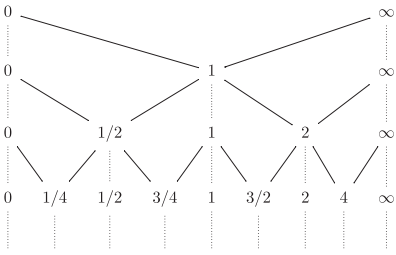
\includegraphics{slike/uvodni_primer_drevo.png}
    \caption{Vzeto iz~\cite{osnovni_clanek}}
    \label{uvodni_primer_drevo}
\end{figure}

Opazimo (in tudi vemo), da sta $ x $- in $ y $-osi asimptoti na graf $ f $, torej nekakšni tangenti na $ f $ v točkah $ 0 $ in $ \infty $ (slednja seveda ni točka). Generiramo novo tangento na graf $ f $ v prvi točki drevesa, ki leži med $ 0 $ in $ \infty $. Te tri tangente se sekajo in skupaj tvorijo trikotnik, ki leži pod grafom $ f $, in pokriva del območja prvega kvadranta. Postopek ponovimo, le da sedaj trikotnike tvorimo v do sedaj s trikorniki še nepokritem območju -- vzamemo tangente v naslednjih točkah v drevesu: $ 1/2 $ in $ 2 $. Dobimo trikotnike, kot kaže slika~\ref{uvodni_primer_prvi_trikotniki}. V naslednjem koraku bi vzeli tangente v naslednjih štirih točkah: $ 1/4 $, $ 3/4 $, $ 3/2 $ in $ 4 $. S ponavljanjem postopka v limiti trikotniki pokrijejo celotno območje pod grafom funkcije $ f $.

\begin{figure}[h]
    \centering
    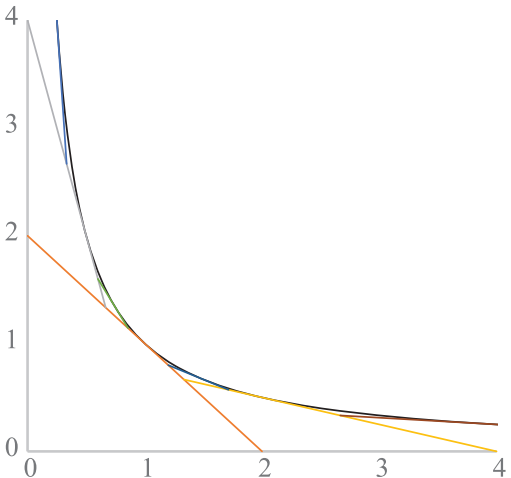
\includegraphics[width=0.3\textwidth]{slike/uvodni_primer_prvi_trikotniki.png}
    \caption{Prve tri tangente v particiji območja na trikotnike. Vzeto iz~\cite{osnovni_clanek}}
    \label{uvodni_primer_prvi_trikotniki}
\end{figure}

Kratek izračun pokaže, da je ploščina vseh trikotnikov, ki z eno stranico ležino na eni od koordinatnih osi (razen prvega trikotnika z ogliščem v izhodišču) konstantna z vrednostjo $ 2/3 $. Iz tega sledi, da je ploščina pod območjem (ki je vsota ploščin vseh trikotnikov) navzgor neomejena, saj je divergentna že vsota ploščin trikotnikov ob oseh. To je v skladu z vrednostjo izlimitiranega integrala $ \int_{0}^{\infty}\frac{1}{x}dx $. S tem načinom razdelitve območja na trikotnike lahko povežemo območje pod grafom in neskončno vrsto, ki ustreza ploščini teh trikotnikov.

Sedaj lahko raziščemo obnašanje teh vrst na primerih različnih funkcij in na različnih števnih gostih podmnožic.




%%%%%%%%%%%%%%%%%%%%%%%%%%%%%%%%%%%%%%%%%%%%%%
\section{Splošnejša obravnava problema}

Pri Riemannovem integralu poskrbimo za vedno finejšo particijo intervalov, ki ustvari pravokotna območja, ki v limiti skupaj tvorijo območje pod grafom. Naš pristop je podoben, le da mora biti zaporedje particij dovolj urejeno, da lahko dobimo ustrezne trikotnike. Le-to pa omogoča neskončno binarno drevo.

Z določanjem zaporedja particij iz drevesa naš proces generiranja trikotnikov, ki napolnijo območje pod grafom funkcije $ f $, potrebuje le nekaj ključnih predpostavk:

\begin{enumerate}
    \item \label{predpostavka_1} Funkcija $ f $ je definirana na intervalu oblike $(0, \infty)$, $[0,\infty)$, $(0,a]$ ali $[0,a]$, kjer je $ 0 < a < \infty $, in ????????????? sta $x$- in $y$-os tangentni nanjo v točki 0 ter (če imamo končen interval) $a$, ali pa sta ena ali obe osi njeni asimptoti.
    \item \label{predpostavka_2} Funkcija $ f $ je dvakrat zvezno odvedljiva, strogo monotono padajoča ($ f'(x) < 0 $) in strogo konveksna ($ f''(x) > 0 $) za vsak $ x \in A$ (razen krajišči), kjer je $ A $ interval oblike, kot ga navaja točka~\ref{predpostavka_1}.
    \item \label{predpostavka_3} Množica, generirana iz neskončnega binarnega drevesa, je gosta podmnožica intervala $ A $.
\end{enumerate}

Te tri predpostavke so dovolj. Predpostavka~\ref{predpostavka_1} zagotavlja, da bosta dve stranici prvega trikotnika ležali na koordinatnih oseh. Predpostavka~\ref{predpostavka_2} poskrbi, da se novo generirane tangente tako razlikujejo od tangent iz prejšnjega koraka, da se tretja stranica novega trikotnika ne prekriva s prejšnjimi, sam trikotnik pa leži pod grafom. Predpostavka~\ref{predpostavka_3} pomeni, da se bo vsaka točka $ (x_0, y_0) $ v prvem kvadrantu, ki leži pod grafom, nahajala v vsaj kakšnem trikotniku.

Računanje ploščine kateregakoli od teh trikotnikov je preprost izračun. Za primer vzemimo tri zaporedne točke iz nekega istega nivoja drevesa: $ 0 < x_1 < x_{1,2} < x_2 $. Točka $ x_{1,2} $ je generirana iz prejšnjih zaporednih točk $ x_1 $ in $ x_2 $. Znamo izračunati tangente na graf $ f $ v teh treh točkah ter medsebojna presečišča, kar so ravno vsi trije vrhovi novega trikotnika. Njegovo ploščino pa izračunamo iz vektorskega produkta poljubnih dveh vektorjev, ki iz enega vrha določata dve stranici tega trikotnika. V konkretnem primeru je računanje dokaj enostavno, v splošnem pa je ploščina tega trikotnika enaka 

\begin{equation}
    \label{splosna_ploscina_formula}
    P = \frac{A^2}{2B}\text{,}
\end{equation}

kjer sta

\begin{align*}
    A =  &f'(x_1)f'(x_{1,2})(x_1 - x_{1,2}) + f'(x_1)f'(x_2)(x_2 - x_1) \\
&+ f'(x_2)f'(x_{1,2})(x_{1,2} - x_2) + f(x_1)(f'(x_2) - f'(x_{1,2})) \\
&+ f(x_2)(f'(x_{1,2}) - f'(x_1)) + f(x_{1,2})(f'(x_1) - f'(x_2))
\end{align*}

in
$$
B = (f'(x_1) - f'(x_{1,2}))(f'(x_1) - f'(x_2))(f'(x_2) - f'(x_{1,2}))\text{.}
$$

\begin{figure}[h!]
    \centering
    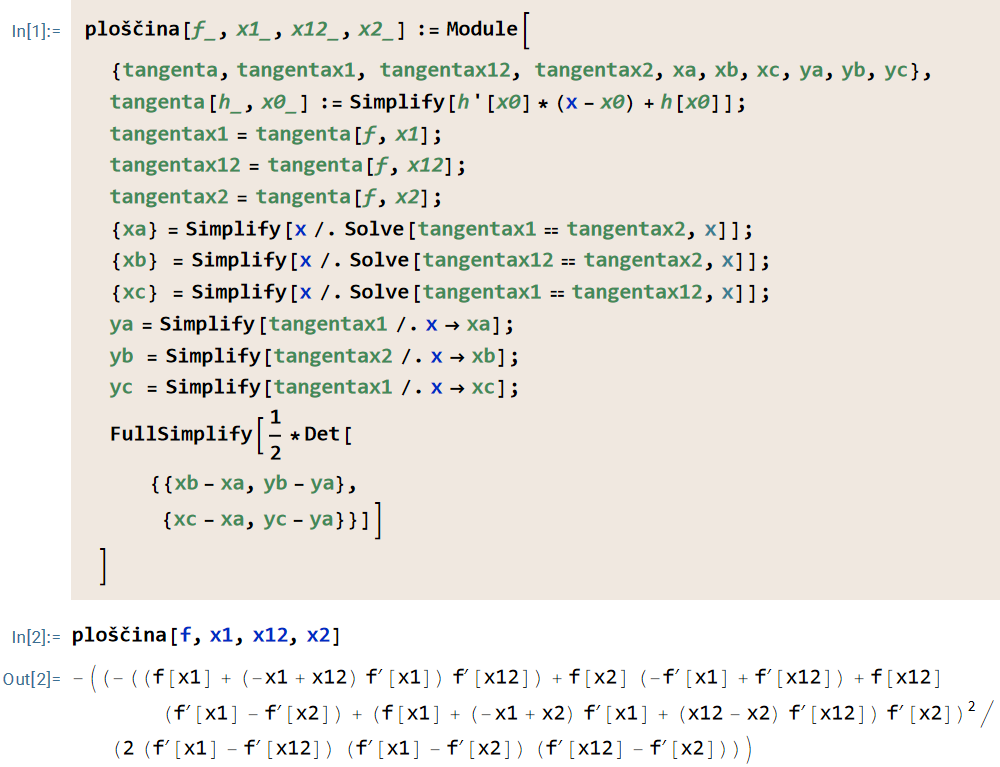
\includegraphics[width=0.8\textwidth]{slike/splosna_ploscina.png}
    \caption{Primer funkcije v programu Wolfram Mathemtatica, ki izračuna splošno ploščino (pod predpostavko, da se vse tri tangente paroma sekajo).}
    \label{splosna_ploscina}
\end{figure}


%%%%%%%%%%%%%%%%%%%%%%%%%%%%%%%%%%%%%%%%%%%%%%
\section{Ilustrativen primer} \label{ilustrativen_primer}

Vzemimo funkcijo $ g(x) = (1 - \sqrt{x})^2 $ na $ [0, 1] $ in drevo, ki ga prikazuje slika~\ref{ilustrativen_primer_drevo}. Nekoliko je podobno drevesu iz uvodnega primera.

\begin{figure}[h]
    \centering
    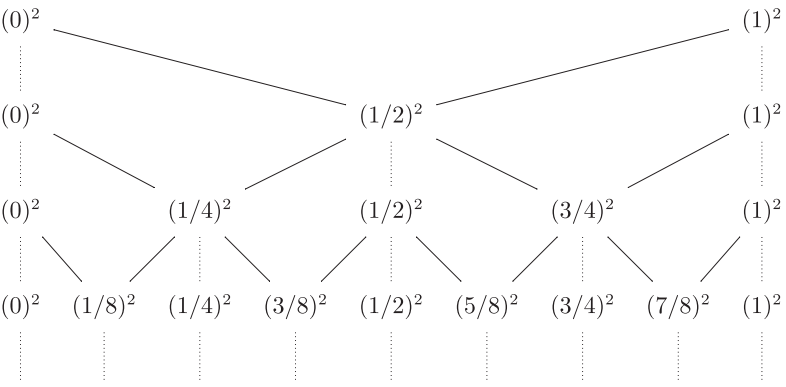
\includegraphics[width=0.7\textwidth]{slike/ilustrativen_primer_drevo.png}
    \caption{Vzeto iz~\cite{osnovni_clanek}}
    \label{ilustrativen_primer_drevo}
\end{figure}

Zlahka preverimo, da za $ g $ in to drevo veljajo vse tri potrebne predpostavke. Radi bi izračunali ploščino pod grafom funckije $ g $ preko trikotnikov (z Riemannovim integralom dobimo rezultat 1/6).

Označimo nivoje drevesa z $ n $. Nivo $ 0 $ sta točki $ (0)^2 $ in $ (1)^2 $, nivo $ 1 $ točke $ (0)^2 $, $ \bigl(\frac{1}{2}\bigr)^2 $ in $ (1)^2 $, nivo $ 2 $ točke $ (0)^2 $, $ \bigl(\frac{1}{4}\bigr)^2 $, $ \bigl(\frac{1}{2}\bigr)^2 $, $ \bigl(\frac{3}{4}\bigr)^2 $, in $ (1)^2 $, \ldots v splošnem torej nivo $ n $ predstavljajo točke $ (0)^2 $, $ \bigl(\frac{1}{2^n}\bigr)^2 $, $ \bigl(\frac{2}{2^n}\bigr)^2 $, $ \bigl(\frac{3}{2^n}\bigr)^2 $, \ldots, $ \bigl(\frac{2^n-2}{2^n}\bigr)^2 $, $ \bigl(\frac{2^n-1}{2^n}\bigr)^2 $ in $ (1)^2 $. Z vsakim nivojem dobimo nove točke, s tem pa tudi nove trikotnike -- natančneje, v nivoju n generiramo $ 2^{n-1} $ novih točk/trikotnikov.

Izkaže se, da je ploščina trikotnikov, ki jih dobimo v vsakem nivoju, enaka in odvisna le od $ n $. Do nje pridemo postopoma: najprej premislimo, da je vsak nov trikotnik v nivoju $ n $ odvisen od treh sosednjih točk na tem nivoju, od katerih je srednja tista, ki je na novo generirana. Tako lahko nivo $ n $ razdelimo na $ 2^{n-1} $ trojic: $ \{(0)^2, \bigl(\frac{1}{2^n}\bigr)^2,\bigl(\frac{2}{2^n}\bigr)^2\} $, $ \{\bigl(\frac{2}{2^n}\bigr)^2, \bigl(\frac{3}{2^n}\bigr)^2, \bigl(\frac{4}{2^n}\bigr)^2\} $, \ldots, $ \{\bigl(\frac{2^n-2}{2^n}\bigr)^2, \bigl(\frac{2^n-1}{2^n}\bigr)^2, (1)^2\}$. Označimo s $ k $ zaporedno mesto novo generirane točke v $ n $-tem nivoju, torej $ k = 1, 3, 5, \ldots, 2^n-1 $. Za vsak $ k $ lahko s pomočjo formule~\ref{splosna_ploscina_formula} izračunamo ploščino novega trikotnika, ki ima za oglišča presečišča tangenta v točkah $ \{\bigl(\frac{k-1}{2^n}\bigr)^2, \bigl(\frac{k}{2^n}\bigr)^2, \bigl(\frac{k+1}{2^n}\bigr)^2\} $. Ploščina je res neodvisna od $ k $ in znaša $ \frac{1}{2^{3n}} $.

Sedaj lahko izračunamo ploščino pod grafom funkcije $ g $. Trikotnike dobimo od nivoja $ 1 $ naprej, zato je $ n = 1, 2, 3, 4, \ldots $. Na $ n $-tem koraku dobimo $ 2^{n-1} $ novih trikotnikov s ploščino $ \frac{1}{2^{3n}} $. Premisliti moramo le uvedbo nove spremenljivke, ki bo namesto $ k $ tekla po zaporednih celih številih: vzamemo npr. $ t = \frac{k-1}{2} $, torej $ t = 0, 1, 2, 3, \ldots, 2^{n-1}-1 $. Ploščina pod grafom je tako res enaka

\begin{equation*}
    \sum_{n=1}^{\infty} \sum_{t=0}^{2^{n-1}-1} \frac{1}{2^{3n}} = \sum_{n=1}^{\infty} \frac{2^{n-1}}{2^{3n}} = \sum_{n=1}^{\infty} \frac{1}{2^{2n+1}} = \sum_{n=0}^{\infty} \frac{1}{2^{2n+3}} = \frac{1}{2^3} \frac{1}{1-\frac{1}{2^2}} = \frac{1}{6}\text{.}
\end{equation*}

\begin{figure}[h!]
    \centering
    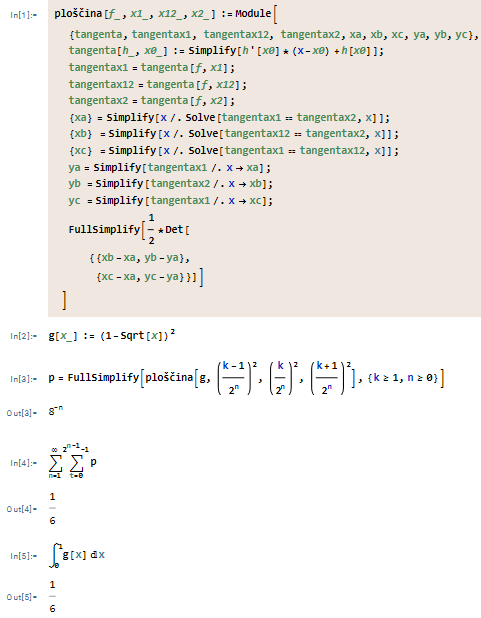
\includegraphics[width=0.8\textwidth]{slike/ilustrativen_primer_wolfram.png}
    \caption{Izračun ploščine trikotnikov iz $ n $-tega nivoja danega drevesa ter celotna ploščina pod območjem funkcije $ g $.}
    \label{ilustrativen_primer_wolfram}
\end{figure}

Ta primer med drugim tudi prikazuje še en način generiranja gostih podmnožic domene funkcije.

%%%%%%%%%%%%%%%%%%%%%%%%%%%%%%%%%%%%%%%%%%%%%%
\section{Generiranje gostih podmnožic z uporabo \\ Stern-Brocotovega drevesa}


\newpage
%%%%%%%%%%%%%%%%%%%%%%%%%%%%%%%%%%%%%%%%%%%%%%
\section{Zaključek}

KAKO PA GENERIRAMO TA DREVESA??? JE USELIH????

\newpage
%%%%%%%%%%%%%%%%%%%%%%%%%%%%%%%%%%%%%%%%%%%%%%
\newpage
\nocite{*}      % navede tudi vire, ki jih ne citiras
\printbibliography
%%%%%%%%%%%%%%%%%%%%%%%%%%%%%%%%%%%%%%%%%%%%%%
\end{document}